\chapter{Methodology}
\label{chapter:methodology}

\section{Architecture Overview}
\label{section:architecture_overview}

In this section, I propose a new model for single-concept open-ended visual question answering tasks. The proposed model comprises six main components, as shown in \figureautorefname{ \ref{fig:model_overview}} and outlined briefly below:

\begin{figure}[htbp]
    \centering
    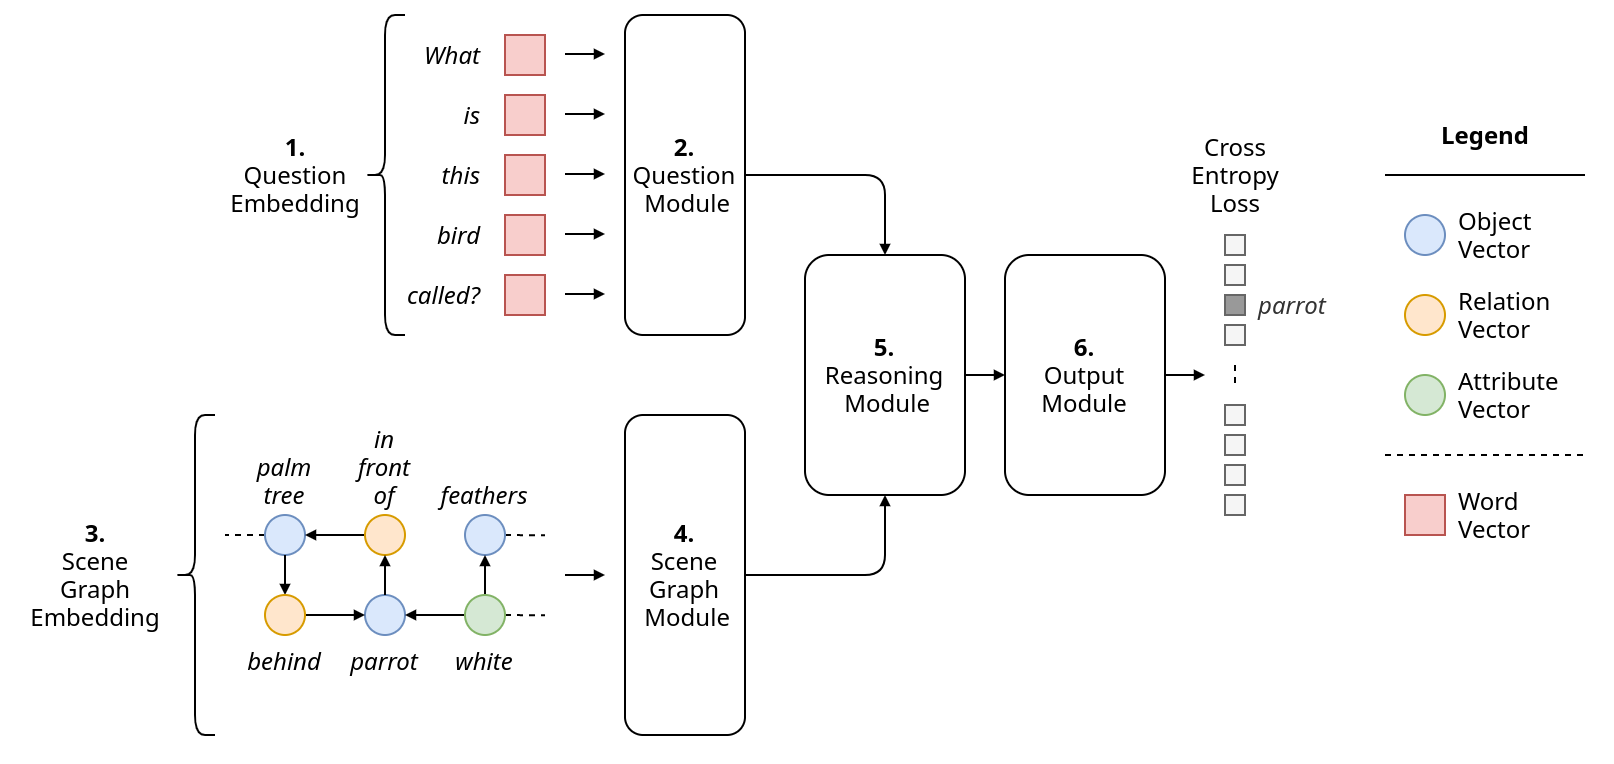
\includegraphics[width=\textwidth]{model_overview.png}
    \caption{A high-level overview of the proposed visual-question-answering model.}
    \label{fig:model_overview}
\end{figure}

\textbf{Question embedding:} In classic NLP fashion, the question embedding component is responsible for the preprocessing and vectorisation of raw question data for use by the rest of the model.

\textbf{Question module:} The question module has two main roles: the first is to learn a sequence of contextual words {\color{red}(TODO: Insert nomenclature)} that capture the relevant features of each question word in the context of the question as a whole. Secondly, the question module learns a question-level embedding that contains information about the question as a whole.

\textbf{Scene graph embedding:} The scene graph embedding model is responsible for the preprocessing and vectorisation of scene graph data. In this dissertation, we use ground-truth scene graphs from the GQA in order to evaluate the effectiveness of sparse graph-based models, however this component can be readily extended to utilise the output of existing scene graph generation models, giving rise to a true end-to-end VQA model.

\textbf{Scene graph module:} The primary goal of the scene graph module is to learn a dense representation of scene graph features that can be used as a knowledge-base for the reasoning module to draw information from when answering questions.

\textbf{Reasoning module:} Given the output features of the scene graph and question modules, the reasoning module is in charge of determining which visual features are relevant to the question and vice-versa. The reasoning capabilities of many existing VQA models could be leveraged here; I justify my reasoning module of choice and describe its implementation in detail in \sectionautorefname{ \ref{section:reasoning_module}}.

\textbf{Output module:} The output module is the simplest part of the architecture, and is responsible for transforming the output of the reasoning module into a concrete answer to the input question. I delve into the design decisions behind the output module and how it might be modified for other VQA tasks in \sectionautorefname{ \ref{section:output_module}}.

\section{Question Embedding}
\label{section:question_embedding}

The question embedding component of the architecture is responsible for two major tasks: preprocessing and vectorisation. The preprocessing step is performed prior to the training of the model, where vectorisation of preprocessed question words occurs at runtime. 

I use a neural preprocessing pipeline for each raw question string in the dataset, comprising tokenisation, part-of-speech (POS) tagging, lemmatisation and dependency parsing steps.\footnote{For this architecture, only the tokenisation step is required since the question module uses word embeddings but not syntactic dependency information. Graph-based question modules use syntactic dependencies for graph construction, as described in \sectionautorefname{ \ref{sec:ablation_studies}}.} For reproducibility, I use the Stanza NLP package \cite{qi2020stanza} for all steps of the pipeline.

After tokenisation, each question token is converted to an index to enable vector embedding lookups during training. A mapping of all question tokens to their respective indices is kept, and shared between the training and validation sets. Reference answers are converted to indices in a similar fashion, however they are not tokenised first. Multi-word answers like \textit{parking meter} or \textit{cutting board} are treated as a single concept, identically to single-word answers like \textit{bed}. This ensures  multi-word answers can be predicted just as easily as single-word answers and allows the output module to treat the question-answering task as a multi-class classification problem across the set of all candidate answers.

At runtime, each question token is converted to a \(d = 300\) dimensional GloVe vector \cite{pennington2014glove}, then token embeddings for a given question are stacked together, yielding a matrix of question features \(h_q \in \R^{l_q \times d}\) where \(l_q\) is the number of tokens in the question. For a batch of questions \(\{q_1, ..., q_n\}\) the corresponding features \(\{h_{q_1}, ..., h_{q_n}\}\) are padded with zeros along the first dimension and then stacked to yield a batch of question features \(H_Q \in \R^{n \times l \times d}\), where \(l = \max_{i} l_{q_i}\). \(H_Q\) is the output of the question embedding module and the input to the question module.

\section{Question Module}
\label{section:question_module}

BiLSTM \cite{hochreiter1997long}

I describe variations of the question module in \sectionautorefname{ \ref{sec:ablation_studies}}.


\section{Scene Graph Embedding}
\label{section:scene_graph_embedding}

 Both the GQA and CLEVR datasets contain ground-truth scene graph information for each image in the training and validation sets. For GQA, each image is annotated with a global \texttt{location} and \texttt{weather} attribute,  as well as a list of objects, the objects attributes \textit{e.g.} colour, shape, texture and its relations to other objects in the image.

\section{Scene Graph Module}
\label{section:scene_graph_module}

{\color{red} TODO: Verify this still holds: Interestingly, using non-linearities such as ReLU between GAT convolutions destroys the rich information provided by the GloVe embeddings by setting negative values to zero.}

\section{Reasoning Module}
\label{section:reasoning_module}

{\color{red}Partly chose MAC network since is is already well-evaluated on the GQA dataset.}

Given the goal of the question module is to learn a dense contextual and syntactic representation of the question, and the goal of the scene graph module is to capture dependency information between objects, attributes and relations in the scene, we still need to combine and reason about this extracted information. All VQA models have to handle this multi-modal fusion and reasoning in some capacity, with adopting taking fusion-only approaches, whilst others learn self-attention or bidirectional attention weights between question and image modalities, and others leverage the strengths of both methods. For my model, I leverage the reasoning capabilities of the Compositional Attention Network \citeauthor{hudson2018compositional}, a recurrent model that decomposes complex question-answering problems into discrete reasoning steps, each of which is performed by a single cell in the network. The Compositional Attention Network achieved state-of-the-art results on the CLEVR dataset in \citeyear{hudson2018compositional}, achieving 

In order to leverage the computational benefits of sparse tensor operations implemented in PyG \cite{fey2019fast}, I used a PyTorch \cite{paszke2019pytorch} re-implementation of the MAC network, which has been trained to 98.6\% on the CLEVR dataset \cite{eyzaguirre2020differentiable}, just 0.3\% shy of the official result reported by 
\citeauthor{hudson2018compositional}. Notably, this re-implementation accounts for minor details that were omitted from the original MAC network paper but enabled by default in the official MAC network repository {\color{red} citation required}.



\section{Output Module}
\label{section:output_module}

\begin{figure}[htbp]
    \centering
    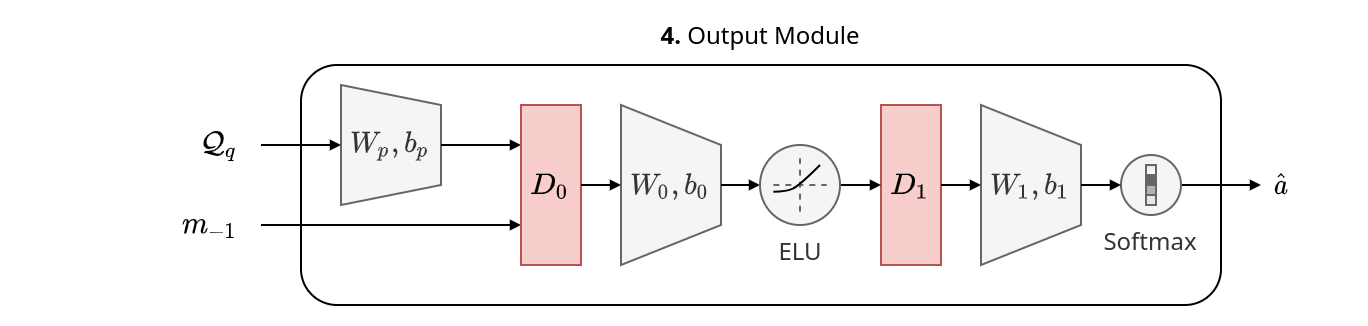
\includegraphics[width=\textwidth]{output_module.png}
    \caption{An overview of the output module, as implemented in the original P}
    \label{fig:output_module}
\end{figure}

{\color{red}

Move to Ablations

\begin{itemize}
  \item Concat + linear fusion (other fusion types?)
  \item Bottom-up
  \item MAC network
\end{itemize}

\subsection{Bottom-up}
\label{subsection:bottom_up}
 ReLU proved to yield higher results over gated tanh when paired with GAT/GCN embeddings. In the original paper, CNN/R-CNN features are extracted in the preprocessing step, meaning there is no need for gradient propagation to the knowledge base embedding. Preliminary tests showed a need for learnable embeddings in graph convolutional models, and thus a need for end-to-end propagation of gradients.}



\begin{itemize}
  \item Initial tests showed little performance difference between conditioning the current control state on previous control states. % #TODOInvestigate interpretability effects
\end{itemize}
